
% \abstract{
% In this study we present a non-overlapping Schwarz waveform relaxation (SWR) method
% applied to a one dimensional model problem representative of the coupling between 
% the ocean and the atmosphere. This problem includes nonlinear interface conditions 
% analogous to a quadratic friction law. We study the convergence of the corresponding 
% SWR at a semi-discrete level for a linear friction and for a linearized quadratic
% friction at the interface. Using numerical experiments we show that the convergence 
% properties in the linearized quadratic friction case are very close to the ones 
% obtained with the full nonlinear problem for the range of parameter values of 
% interest. We investigate the possibility to improve the convergence speed by 
% adding a relaxation parameter at the interface.}

\section{Introduction}
We presented in Chapter \ref{ch:discreteSchwarzAnalysis}
the discrete analysis of the convergence of Schwarz methods;
the implementation of the law of the wall was discussed
in Chapter \ref{ch:ND}. We now aim to study the convergence
properties of Schwarz methods when the law of the wall is
used at the interface between ocean and atmosphere.
In this chapter, we study the Ekman problem with a
simplified bulk condition at the surface such that
it can be easily implemented to numerically validate the
convergence results.
A part of this chapter was published in proceedings of the
International Conference on Domain Decomposition Methods
\citep{clement_discrete_2021}.

Schwarz-like domain decomposition methods are very popular in 
mathematics, computational sciences and engineering notably for 
the implementation of coupling strategies. Such an iterative method
has been recently applied in a state-of-the-art Earth 
System Model (ESM) to evaluate the consequences of inaccuracies 
in the usual ad-hoc ocean-atmosphere coupling algorithms 
used in realistic models \cite{marti_schwarz_2021}. For such 
a complex application it is challenging to have an a priori 
knowledge of the convergence properties of the Schwarz method. 
Indeed coupled problems arising in ESMs often 
exhibit sharp turbulent boundary layers whose parameterizations 
lead to peculiar transmission conditions. The objective in
this paper is to study a model problem representative 
of the coupling between the ocean and the atmosphere, including discretization 
and so-called bulk interface conditions which are analogous to a 
quadratic friction law. Such a model is introduced in Section \ref{sec:couplingProblem}
and its discretization, as done in state-of-the-art ESMs, 
is described in Section \ref{sec:discreteProblem}. In the semi-discrete
case in space we conduct in Section \ref{sec:conv-lin} a convergence analysis 
of the model problem first with a linear friction and then with a 
quadratic friction linearized around equilibrium solutions. 
Finally, in Section \ref{sec:num-exp}, numerical experiments in the 
linear and nonlinear case are performed to illustrate the relevance 
of our analysis. \par
%
\section{Model problem for ocean-atmosphere coupling}\label{sec:couplingProblem}
%===============================================================
We focus on the dynamical part of the oceanic and atmospheric primitive equations and neglect the horizontal variations of 
the velocity field, which leads to a model problem  depending 
on the vertical direction only. This assumption, commonly made 
to study turbulent mixing in the boundary layers near the 
air-sea interface, is justified because of the large disparity 
between the vertical and the horizontal spatial scales in these layers. 
We consider the following diffusion problem accounting for Earth’s 
rotation ($f$ is the Coriolis frequency and $\mathbf{k}$ a vertical unit vector):
%===============================================================
\begin{equation*}
\left\{
\begin{array}{rcll}
\partial_t \mathbf{u} + f \mathbf{k} \times \mathbf{u} - \partial_z \left( \nu(z,t) \partial_z \mathbf{u} \right) &=& \mathbf{g}, & \mbox{in}\;\Omega \times (0,T), \\
\mathbf{u}(z,0) &=& \mathbf{u}_0(z), & \forall z \; \mbox{in}\; \Omega, \\
\mathbf{u}(H_o,t) &=& \mathbf{u}_o^\infty(t), ~ \mathbf{u}(H_a,t) = \mathbf{u}_a^\infty(t), ~ & t \in (0,T),  
\end{array}
\right.
\end{equation*}
%===============================================================
with $\mathbf{u} = (u,v)$ the horizontal velocity vector,
$\nu(z,t) > 0$ the turbulent viscosity and 
$\Omega = (H_o,H_a)$ a bounded open subset of $\mathbb{R}$
containing the air-sea interface $\Gamma = \{z = 0\}$.
In the ocean and the atmosphere, which are  turbulent fluids,
the velocity field varies considerably in the few 
meters close to the interface (in a region called 
\textit{surface layer}). The cost of an
explicit representation of the surface layer in numerical simulations being 
unaffordable, this region is numerically accounted for 
using wall laws a.k.a. log laws (e.g. \cite{mohammadi_rough_1998}). This approach, 
traditionally used to deal with solid walls, is also used
in the ocean-atmosphere context, with additional complexity 
arising from the stratification effects \cite{pelletier_two-sided_2021}.
In this context wall laws are referred to as \textit{surface layer} 
parameterizations. The role of such parameterizations is to provide 
$\nu \partial_z \mathbf{u}$ on the upper and lower interfaces of the 
surface layer as a function of the difference of fluid velocities.
Thus the coupling problem of interest should be understood as a domain
decomposition with three non-overlapping subdomains. For the sake 
of convenience the velocity vector $\mathbf{u} = (u,v)$ 
is rewritten as a complex variable $U = u + i v$. Then the model problem reads   
%===============================================================
\begin{equation}
\label{eq:cplProblem}
%\left\{
\begin{array}{rcll}
\partial_t U_j + i f U_j - \partial_z \left( \nu_j(z,t) \partial_z U_j \right) &=& g_j,
~~~~~~~~~~ (j=o,a)
& \mbox{in}\;\Omega_j \times (0,T)\\
U_j(H_j,t) &=& U_j^\infty(t),  & t \in (0,T), \\ 
U_j(z,0) &=& U_0(z), & \forall z \; \mbox{in}\; \Omega_j, \\
\rho_o \nu_o \partial_z U_o(\delta_o,t) = \rho_a \nu_a \partial_z U_a(\delta_a,t)
&=& {\cal F}_{\rm sl}( U_a(\delta_a,t)-U_o(\delta_o,t) ), \;\; & t \in (0,T)
\end{array}
%\right.
\end{equation}
%===============================================================
%\begin{subequations}\label{eq:cplProblem}
%\begin{align}
%\partial_t \psi_j + i f \psi_j - \partial_x \left( \nu_j(x,t) \partial_x \psi_j \right) %&= g_j, & \mbox{in}\;\Omega_j \times (0,T),\\
%\psi_j(H_j,t) &= \psi_j^\infty(t),  & t \in (0,T), \\ 
%\psi_j(x,0) &= \psi_0(x), & \forall x \; \mbox{in}\; \Omega_j, \\
%\rho_o \nu_o \partial_x \psi_o(\delta_o,t) = \rho_a \nu_a \partial_x \psi_a(\delta_a,t)
%&= {\cal F}_{\rm sl}( \psi_a(\delta_a,t)-\psi_o(\delta_o,t) ), \;\; & t \in (0,T)
%\end{align}
%\end{subequations}
%===============================================================
where $\Omega_o= (H_o,\delta_o)$, $\Omega_a = (\delta_a,H_a)$, and 
${\cal F}_{\rm sl}$ is a parameterization function for the surface layer 
extending over $\Omega_{\rm sl} = (\delta_o,\delta_a)$. A typical 
formulation for ${\cal F}_{\rm sl}$ is
\[
{\cal F}_{\rm sl}( U_a(\delta_a,t)-U_o(\delta_o,t) ) = 
\rho_a C_D | U_a(\delta_a,t)-U_o(\delta_o,t) | (U_a(\delta_a,t)-U_o(\delta_o,t))
\]
which corresponds to a quadratic friction law with $C_D$ 
a drag coefficient (assumed constant in the present study).
%
%
%To study the coupling problem as a one-dimensional coupling,
Geostrophic winds and currents are used in this study as
source terms and boundary conditions. 
Geostrophic equilibrium is the steady state for which the 
Coriolis force compensates for the effects of gravity.
It corresponds to the large scale dynamics of ocean and 
atmosphere, and leads to reasonable values of the solution $U$. \par
%In the following, geostrophic fields are  supposed to be independent 
%of $z$ in each subdomain: $U_j^\infty$ and $U_0(z)$
%are hence set to constant values of $10\;{\rm m.s^{-1}}$ in the 
%atmosphere and $0.1\;{\rm m.s^{-1}}$ in the ocean. Forcing term 
%$g_j$ is set to $i f U_0 (z)$.\par
The well-posedness of \eqref{eq:cplProblem} has been studied in 
\cite{thery_etude_2021}
%\cite{thery_etude_2021} studied the well-posedness of \eqref{eq:cplProblem}. 
where it is proved that its steady version admits a unique
solution for realistic values of the parameters. The study of the
nonstationary case is much more challenging: numerical experiments
tend to confirm this well-posedness and we give in Section
\ref{sec:OASchwarz_wellPosedness} some elements for a theoretical proof.
%
%
%
%a method traditionally used to deal with 
%
%
%for turbulent 
%flows near interfaces 
%
%wall laws are traditionally used 
%for turbulent flows near interfaces
%
%
%\newpage 
%
%\cite{thery_etude_2021}
%\cite{Pelletier_etal_2021}
% 
%The ocean-atmosphere system can be represented in the vertical direction by a coupling %between three main areas of interest: \textcolor{blue}{Simon: Plutôt un schéma comme dans %le début de la thèse de Sophie ?}
%\begin{itemize}
%    \item A surface boundary layer, including a turbulent zone and a viscous sublayer on %each side side of the air-sea interface.
%    \item The domain of the atmosphere above the surface boundary layer
%    \item The ocean domain under the surface boundary layer
%\end{itemize}
%
%
%\section{Well-posedness} \label{sec:wellPosed}

%Heat and momentum involved in air-sea exchanges 
%are displaced away from the interface by the turbulent motions. Because the %vertical resolution
%of climate models is much finer than the horizontal, the turbulent mixing can be viewed as a one-dimensional diffusion equation.

%To study the convergence of Schwarz Waveform Relaxation applied to the ocean-atmosphere coupling, we use two coupled diffusion equations
%\begin{equation} \label{eq:innerDiffusionEq}
%\begin{aligned}
%    \partial_t u_{\rm o} (x,t) - \partial_x \left(\nu_{\rm o} \partial_{x} u_{\rm o} (x, t)\right) &=0, ~~~ x \in (-\infty, 0], ~~~ t\in [0,T)
%    \\
%    \partial_t u_{\rm a}(x,t) - \partial_x \left( \nu_{\rm a} \partial_{x} u_{\rm a}(x,t) \right) &=0, ~~~ x \in [0, +\infty), ~~~ t\in [0,T)
%\end{aligned}
%\end{equation}
%where the subscript ${\rm o}$ stands for \textit{ocean} and ${\rm a}$ for \textit{atmosphere}. 
%We choose flux transmissions between the two
%domains $\mathbb{R}_{-}$ and $\mathbb{R}_{+}$ similar to the air-sea exchanges in climate models.

%The air-sea fluxes are usually estimated through bulk formulations: empirical formulae such that
%data at reference levels can give the fluxes without knowing the full profile of the variables.
%Bulk formulations are used both to extrapolate measurement to sea surface and to enhance
%numerical simulations. The reference levels are typically of ${\rm 10\; m}$ above the sea surface in the atmosphere and ${\rm 1\; m}$ under the interface in the ocean.

%Our coupling problem will be consisted of \eqref{eq:innerDiffusionEq}, of initial value and boundary conditions, and of the coupling conditions
%\begin{equation}\label{eq:couplingConditions}
%    \frac{\rho_{\rm o}}{\rho_{\rm a}}\nu_{\rm o} (\partial_x u_{\rm o})(x=0)
%    =(\nu_{\rm a} \partial_x u_{\rm a})(x=0)
%    = \alpha \left(
%    u_{\rm a}(x=h_{\rm a}/2) - u_{\rm o}(x=-h_{\rm o}/2)
%    \right)
%\end{equation}
%where $\rho_{\rm o}$ and $\rho_{\rm a}$ are respectively the density of water and of air at sea surface.
%The left equality ensures the equality between the flux of the considered variable while
%the right equality links the jump of the variable to the flux. The possible values of $\alpha$ are detailed in section \ref{subsec:heat} and \ref{subsec:momentum}.
%Note that we study one variable at a time,
%which makes our transmission conditions very different from the actual bulk formulations used in climate models \cite{taylor2000intercomparison}.
%However, we are not concerned here by the accuracy but by the convergence speed. 
%The analysis of such a coupled problem is inherently discrete, as it uses the prognostic variables at the first height level of each model.
%
% where $\alpha$ either depends on 
% $||u_{\rm a,10} - u_{\rm o,-1} ||$ (\textit{nonlinear} case, close to the momentum condition)
% or is independant of $u$ (\textit{linear} case, close to the heat condition when heat and momentum are decoupled)
% The analysis of such a coupled problem is inherently discrete, as it uses the prognostic variables at the first height level of each model.



%\subsection{Heat} \label{subsec:heat}
%Sensible heat flux $Q_{\rm s}$ and latent heat flux $Q_{\rm l}$ are estimated through bulk formulae \citep[][]{large2004diurnal}:
%\begin{equation}
%\begin{aligned}
%    \frac{Q_{\rm s}}{\rho_{\rm a}} &= C_p C_s \left|\Delta U\right| (T_{\rm a} - SST) \\
%    \frac{Q_{\rm l}}{\rho_{\rm a}} &= L_E C_L \left|\Delta U \right|\left(q_s - q_a \right)
%\end{aligned}
%\end{equation}
%where $\rho_a$ is the density of air, $C_p$, $C_s$, $L_E$ and $C_L$ are respectively the heat capacity of air ($C_p \approx 1.3 {\rm J(Kkg)^{-1}}$), the sensible heat transfer coefficient ($C_s \approx 900$), the latent heat coefficient ($L_E \approx 2.5 {\rm Jkg^{-1}}$) and the latent heat transfer coefficient ($C_L \approx 1.3\times 10^{-3}$).
%
%$q_s$ is the saturation humidity that depends on the sea surface temperature $SST$ whereas $q_a$ is the humidity at the reference level.
%
%We can hence choose a constant $\alpha$ in \eqref{eq:couplingConditions}
%to have a similar effect to those flux calculations:
%\begin{equation}
%    \alpha_{\rm linear} = \left|\Delta U \right| \left(C_p C_s + L_E C_L\right)
%\end{equation}
%
%
%\subsection{Momentum} \label{subsec:momentum}
%The momentum flux $\nu \partial_x \boldsymbol{u}$
%is usually provided to ocean models as a boundary condition under the form
%\begin{equation}
%    \nu \partial_x \boldsymbol{u} = \frac{\boldsymbol{\tau}}{\rho_{\rm a}}
%\end{equation}
%where $\boldsymbol{\tau}$ is the wind shear and $\rho_{\rm a}$ the density of air close to the surface.
%
%$\boldsymbol{\tau}$ is function of the wind velocity at the reference level of 10 meters above the ocean. The wind velocity is taken relative to the ocean surface velocity \citep[e.g.][]{hersbach2008relevance}.
%
%\begin{equation}
%\tau = \rho_{\rm a} c_D
%\left|\boldsymbol{u_{\rm a}} - \boldsymbol{u_{\rm o}} \right|\left(\boldsymbol{u_{\rm a}} - \boldsymbol{u_{{\rm o}}}\right)
%\end{equation}
%Where $c_D$ is the drag coefficient. It is either
%simplified as a fixed coefficient ($c_D \approx 1.3 \times 10^{-3}$) or assumed to depend on the other variables involved \citep[][]{taylor2000intercomparison}. In this study, we focus on a fixed drag coefficient.
%The corresponding $\alpha$ in \eqref{eq:couplingConditions}
%thus gives a \textit{nonlinear} coupling condition,
%\begin{equation}
%    \alpha_{\rm nonlinear} = c_D \left|u_{\rm a} - u_{\rm o}\right|
%\end{equation}

\section{Discretized coupled problem}\label{sec:discreteProblem}
%==============================================
\subsection{Implementation of the surface layer}
%==============================================
As described in Section \ref{sec:couplingProblem}, the full domain 
$\Omega$ is split into three parts: $\Omega_o$ in the ocean, 
$\Omega_a$ in the atmosphere and $\Omega_{\rm sl}$ a thin domain 
containing the interface (see Fig. \ref{fig:presentationDomains}).
The role of  
$\Omega_{\rm sl}$ is to provide $\rho_j \nu_j \partial_z U_j$ 
at $z=\delta_j$ ($j=o,a$) as a function of fluid velocities at the 
same locations. However, in state-of-the-art climate models, the discretization 
is based on an approximate form of the coupled 
problem \eqref{eq:cplProblem}. For practical reasons, the computational
domains are $\widetilde{\Omega}_o = (H_o,0)=\Omega_o \bigcup (\delta_o, 0)$ and 
$\widetilde{\Omega}_a = (0,H_a) = (0,\delta_a ) \bigcup \Omega_a$, and the locations 
of the lower and upper boundaries of the surface layer ($z=\delta_j$)   
are assimilated to the centers of the first grid cells (i.e. $\delta_o=-h_{\rm o}/2$ 
and $\delta_a=h_{\rm a}/2$ with $h_{\rm o}$ and $h_{\rm a}$ the thicknesses of the first grid cell in each 
subdomain), where the  values of the velocity closest to the interface are available. 
%
%
%and are thus imposed by the vertical grid. 
%coupling problem \eqref{eq:cplProblem} of interest 
%
%The coupling problem \eqref{eq:cplProblem} presented in 
%Section \ref{sec:couplingProblem} is not implemented as is in climate models.
%The bulk parameterization ${\cal F}_{\rm sl}$ is generally included in the atmospheric model. Sea surface fluxes are derived from atmospheric variables at 
%the first atmospheric mesh level ($\approx 10m$), which is thus considered as the top
%of the surface boundary layer $\delta_{\rm a}$, and from oceanic variables at the
%first oceanic mesh level ($\approx 1m$) considered as the bottom
%of the surface boundary layer $\delta_{\rm o}$.
%The vertical variations of oceanic variables in the ocean surface layer are often neglected: the sea surface forcing is directly given to the
%first oceanic mesh level (coinciding approximately with $\sigma_{\rm o} \approx 1m$).
%=========================================================
%The representation of the surface layer is therefore directly dependent of the discretization of oceanic and atmospheric models, and any modification in the vertical resolution of one 
%of the models near the interface leads to an arbitrary change of 
%the thickness of the surface layer. This appears to be a clear weakness 
%of this widely used numerical approach.
%=========================================================
%The fluxes are supposed to be constant in the surface layer, which leads the bulk formula to be discretized as
%
Typical resolutions in the  models are 
$\delta_a=h_{\rm a}/2=10\;{\rm m}$ and $\delta_o=-h_{\rm o}/2=-1\;{\rm m}$.
At a discrete level, the transmission condition in \eqref{eq:cplProblem}
is replaced by
%
\begin{equation}\label{eq:discreteCouplingConditions}
    \rho_{\rm o} \nu_{\rm o} \partial_z U_{\rm o}(0,t)
    = \rho_{\rm a} \nu_{\rm a} \partial_z U_{\rm a}(0,t)
    = \rho_{\rm a} \alpha \left(
    U_{\rm a}\left( \frac{h_{\rm a}}{2},t \right) - U_{\rm o}\left(-\frac{h_{\rm o}}{2},t \right)
    \right)
\end{equation}
%
where 
$\alpha= C_D \left| U_{\rm a}\left( \frac{h_{\rm a}}{2},t \right) - U_{\rm o}\left(-\frac{h_{\rm o}}{2},t \right) \right|$ for the \textit{nonlinear} case.
In the following, for the analysis in Section \ref{sec:conv-lin}, we  consider 
a \textit{linear} friction where $\alpha$ is assumed constant and a 
quadratic friction \textit{linearized} around equilibrium solutions.
\begin{figure}
    \centering
    \includegraphics[scale=1.]{fig_presentation_domains.pdf}
    \caption{Discrete representation of the three domains $\Omega_a, \Omega_{\rm sl}, \Omega_o$ together with a typical steady state. Note the different scales for $(u,v)$ in the ocean and in the atmosphere.}
    \label{fig:presentationDomains}
\end{figure}
\subsection{Schwarz Waveform Relaxation}
As discussed for example in \cite{marti_schwarz_2021},
current ocean-atmosphere coupling methods can actually be seen as a 
single iteration of a Schwarz Waveform Relaxation (SWR) algorithm. 
%In SWR methods, equations on each subdomain are integrated in time 
%alternatively, using at the interface the solution computed previously 
%in the other subdomain. 
SWR applied to the coupling problem presented 
in Section \ref{sec:couplingProblem} with the transmission conditions 
 \eqref{eq:discreteCouplingConditions} and constant viscosity
 in each subdomain reads:
%\begin{subequations}
%\begin{align}
%(\partial_t + if) U^k_j - \nu_j\partial_x \phi^k_j  &= g_j ~~~~~~~~~~~~~~~~~~~~~~~ (x,t) \in \mathbb{R} \times ]0,T]&&\\
%U^k_j(x,t=0) &= U_0(x)   &&  x \in \mathbb{R}  \\
%U^k_j(\pm\infty, t) &= U^\infty_{\rm j} && t \in [0,T]\\
%\nu_{\rm o}\phi^k_{\rm o}(0^-,t) &= (\rho_{\rm a}/\rho_{\rm o})
%\nu_{\rm a}\phi^k_{\rm a}(0^+,t) && t \in [0,T] \label{eq:fluxInterfaceCondition}\\
%\nu_{\rm a}\phi_{\rm a}^{k}(0,t) &=  \alpha 
%\left( U_{\rm a}^{k-1+\theta}(h_{\rm a}/2,t) - U_{\rm o}^{k-1}(-h_{\rm o}/2,t)\right) & & t \in [0,T]
%\label{eq:bulkInterfaceCondition}
%\end{align}
%\end{subequations}
%
\begin{subequations}
\label{eq:SWRbulk}
\begin{align}
(\partial_t + if) &U^k_j - \nu_j\partial_z \phi^k_j  = g_j, 
\hspace{3.4cm} \mbox{in}\;\widetilde{\Omega}_j \times (0,T) \label{eq:ref} \\
U^k_j(z,0) &= U_0(z),   \hspace{4.8cm}  \forall z \in \widetilde{\Omega}_j  \\
U^k_j(H_j, t) &= U^\infty_j, \hspace{5.1cm}  t \in [0,T]\\
\nu_{\rm a}\phi_{\rm a}^{k}(0,t) &=  \alpha^{k-1} 
\left( U_{\rm a}^{k-1+\theta}\left(\frac{h_{\rm a}}{2},t\right) - U_{\rm o}^{k-1}\left(-\frac{h_{\rm o}}{2},t\right)\right), 
\hspace{0.12cm} t \in [0,T] \label{eq:bulkInterfaceCondition} \\
\rho_{\rm o} \nu_{\rm o}\phi^k_{\rm o}(0,t) &= \rho_{\rm a}
\nu_{\rm a}\phi^k_{\rm a}(0,t), \hspace{3.98cm} t \in [0,T] \label{eq:fluxInterfaceCondition}
\end{align}
\end{subequations}
%
where $j={\rm a},{\rm o}$, $\phi_j = \partial_z U_j$, and 
$U_{\rm a}^{k-1+\theta} = \theta U_{\rm a}^{k} + (1-\theta) U_{\rm a}^{k-1}$
with $\theta$ a relaxation parameter (interpolation for $0\leq \theta \leq 1$ or extrapolation for $\theta>1$). 
%
%$h_{\rm a}$ and $h_{\rm o}$ are the space grid sizes {\color{red}défini avant ?} .
%$U_{\rm a}^{k-1+\theta}$ is a shortcut for $\theta U_{\rm a}^{k} + (1-\theta) U_{\rm a}^{k-1}$:
%For $0\le \theta \le 1$, $U_{\rm a}^{k-1+\theta}$ is given by 
%an interpolation between current and previous iterations, and for 
%$\theta>1$ it is an extrapolation. 
%{\color{blue} c'est redondant avec la formule, non ?}
%In practice, models use methods similar to $\theta=1$. {\color{red} mais les modèles n'itèrent pas : ça prête à confusion, non ?}
%
At each iteration, \eqref{eq:fluxInterfaceCondition} ensures that the 
kinetic energy is conserved at the machine precision in the coupled 
system which is a major constraint for climate models. 
%Conservation of energy is indeed a major source of concern in  climate models, and coupling routines must be designed accordingly.
In \eqref{eq:bulkInterfaceCondition},
the presence of the parameter $\theta$ makes it resemble to a Dirichlet-Neumann Waveform Relaxation algorithm.
Indeed, if \eqref{eq:bulkInterfaceCondition} is replaced
by $U_{\rm a}^k = \theta U_{\rm o}^{k-1} + (1-\theta) U_{\rm a}^{k-1}$ the DNWR algorithm is retrieved, as examined in the continuous case in \cite{gander_dirichlet-neumann_2014} and in the discrete case in
\cite{meisrimel_time_2020}.
However \eqref{eq:bulkInterfaceCondition}
involves both $\phi_{\rm a}^k$ and 
$U_{\rm a}^{k-1+\theta}$:
the $\theta$ parameter appears thus here within a (close to Robin) condition  
$\nu_{\rm a} \phi_{\rm a}(0) - \alpha \theta U_{\rm a}(h_{\rm a}/2) = \ldots$,
i.e. the relaxation is not performed directly on the converging variable
which leads to convergence properties different from the DNWR case, 
as shown in Section \ref{sec:conv-lin}.
It is important to distinguish between the relaxation
procedure described here and the choice of using an implicit or
explicit interface condition discussed in Section
\ref{sec:ND_NeutralCase_continuousModel}.
The latter refers to changing the time step $t^n$ whereas the former
refers to choosing the iteration step $k$.
\par
%
In the following, centered finite difference schemes in space are used with constant space steps $h_j$.
Derivatives are approximated as $\phi_j(z,t) = \frac{U_j(z+h_j/2,t) - U_j(z-h_j/2, t)}{h_j}$
and the semi-discrete version of \eqref{eq:ref} in the homogeneous case is
\begin{equation}\label{eq:spaceTimeScheme}
	(\partial_t + if) U_{j, m+\frac{1}{2}} (t) = \nu_j \frac{\phi_{j,m+1}(t) - \phi_{j,m}(t)}{h_j}
\end{equation}

\section{Discrete steady state and well-posedness}
\label{sec:OASchwarz_DiscreteStationaryState}
We now interest ourselves to the semi-discrete in space
steady state of \eqref{eq:SWRbulk}.
\paragraph{Special case $f=0$}
If we set to zero the Coriolis parameter,
The flux $\nu_j\phi_j$ is constant in each domain.
If moreover $U_{\rm a}^{\infty} \neq U_{\rm o}^{\infty}$,
because of the interface conditions
the derivatives $\phi_{\rm a}$ and $\phi_{\rm o}$
cannot be equal to zero and $U_j$ are affine.
With spatial domains of finite size, we eventually
find an equation roughly similar to \eqref{eq:mainEqSimplified}.
However, with the infinite domain hypothesis
$\phi_j$ must tend to zero for $z\rightarrow \pm \infty$.
\textbf{There is no stationary solution with infinite domains
for $f=0$}. Note that this is true for both semi-discrete
and continuous cases.
\newline
We now exclude the particular case of a vanishing Coriolis parameter
and interest us only on the case $f\neq 0$.
In this section, we assume that the space domain is sufficiently
large ($H_j \rightarrow \infty$) but the results can be easily
extended to domains of finite size.
\subsection{Resolution in each subdomain}
A discrete analysis of the finite difference scheme \eqref{eq:spaceTimeScheme}
in the frequency domain (see Chapter \ref{ch:discreteSchwarzAnalysis} or
\cite{wu_optimized_2017}) leads to 
$\widehat{\phi}_{{\rm o}, -m}^k = A_k^{\phi} (\lambda_{\rm o}+1)^m$
and
$\widehat{\phi}_{{\rm a}, m}^k = B_k^{\phi} (\lambda_{\rm a}+1)^m$ 
with $\lambda_j = \frac{1}{2}\left(\chi_j - \sqrt{\chi_j} \sqrt{\chi_j + 4}\right)$, 
$\chi_j=\frac{i (\omega+f) h_j^2}{\nu_j}$.
%with $\chi_j=\frac{i (\omega+f) h_j^2}{\nu_j}$, 
and $m$ the space index.
The steady state analysis is identical, except that $\omega$ is set to 0 and that the transmission conditions are not required
to be linear. 
We note $\widetilde{U_j}(z)$ the stationary solution (and $\widetilde{\phi}_j$ its finite difference derivative) and the space discretisation at the first grid level $h_j$ gives:
$\widetilde{U}_j(\delta_j) = g_j \pm \frac{\nu_j\lambda_j}{if h_j} \{A_k^{\phi}, B_k^{\phi}\}_j$

\begin{remark}[\cite{thery_etude_2021}, \S 5.1.3, \S 5.1.4]
We retrieve a solution of the form
$\widetilde{U}_a(\delta a) = g_a - \Psi_a (u^\star)^2 e^{i\theta}$
but $\Psi_j = -\frac{\lambda_j}{if h_j}$ is simpler thanks to the hypotheses of constant diffusivities and infinite domains.
\end{remark}

\subsection{Derivation of the steady state}
\subsubsection{Simplification of the problem}
We interest ourselves in the
value of $A_k^{\phi}, B_k^{\phi}$ at the potential convergence, namely $A_\infty, B_\infty$.
%This subsection derives the steady state. The results are summarized in the subsection \ref{sec:summary_stationnary}.
The first condition of the bulk equation \eqref{eq:fluxInterfaceCondition} gives us $B_\infty = \frac{\rho_{\rm o} \nu_{\rm o}}{\rho_{\rm a} \nu_{\rm a} } A_\infty$
and the non-linear \eqref{eq:bulkInterfaceCondition} gives
\begin{equation} \label{eq:stationaryBulkFirstEq}
    \frac{\rho_{\rm o} \nu_{\rm o}}{\rho_{\rm a} C_D} A_\infty
    =
    \left|
    \left(
    \frac{\rho_{\rm o}}{\rho_{\rm a}}\frac{\nu_{\rm o}\lambda_{\rm a}}{if h_{\rm a}} 
    +\frac{\nu_{\rm o}\lambda_{\rm o}}{if h_{\rm o}} \right) A_\infty
    + (g_{\rm a} - g_{\rm o})
    \right|
    \left(
    \left(
    \frac{\rho_{\rm o}}{\rho_{\rm a}}\frac{\nu_{\rm o}\lambda_{\rm a}}{if h_{\rm a}} 
    +\frac{\nu_{\rm o}\lambda_{\rm o}}{if h_{\rm o}} \right) A_\infty
    + (g_{\rm a} - g_{\rm o})
    \right)
\end{equation}
We simplify the names to get the following problem:
note $d = C_D \left(
    \frac{\lambda_{\rm a}}{if h_{\rm a}} 
    +\frac{\rho_{\rm a}}{\rho_{\rm o}}\frac{\lambda_{\rm o}}{if h_{\rm o}} \right)$ and
$\widetilde{x} = A_\infty \frac{\rho_{\rm o} \nu_{\rm o}}{\rho_{\rm a} C_D}d+\left(g_{\rm a} - g_{\rm o}\right)$.
$\widetilde{x}$ is the difference between the
solutions $\widetilde{U}_j$ at interface
and $d$ is an non-dimensional number that links
$\widetilde{x}$ and $\rho_j \nu_j \widetilde{\phi}_j(0)$
The problem is to find $\widetilde{x}\in \mathbb{C}$ such that
\begin{equation} \label{eq:mainEqSimplified}
    \widetilde{x} - \left(g_{\rm a} - g_{\rm o}\right) = d|\widetilde{x}|\widetilde{x}.
\end{equation}
\begin{remark}
If the infinite domains hypothesis is relaxed, equation \eqref{eq:mainEqSimplified} is retrieved with slightly different $\widetilde{x}$ and $d$.
\end{remark}
Let us now study the real and imaginary parts of $\widetilde{x}=\widetilde{x}_R+i{\widetilde{x}_I}$ and $d={d_R}+i{d_I}$.
\begin{equation}
    \begin{aligned}
    \widetilde{x}_R &= |\widetilde{x}|({d_R} \widetilde{x}_R - {d_I}{\widetilde{x}_I}) +g_{\rm a} - g_{\rm o} \\
    {\widetilde{x}_I} &= |\widetilde{x}|({d_I}\widetilde{x}_R + {d_R}{\widetilde{x}_I})
    \end{aligned}
\end{equation}
A combination (product with ${\widetilde{x}_I}, \widetilde{x}_R$)
between those equations gives
${d_I}\left|\widetilde{x}\right|^3 = \left(g_{\rm a} - g_{\rm o}\right) {\widetilde{x}_I}$ which means that either ${d_I}=\widetilde{x}_I=0$ or ${d_I}\neq 0$ and $\frac{g_{\rm a} - g_{\rm o}}{{d_I}}{\widetilde{x}_I}>0$.
From \eqref{eq:mainEqSimplified}, $\widetilde{x}$ cannot be real because $g_{\rm a} \neq g_{\rm o}$ and $d$ is not real.
We get the equality
$\widetilde{x}_I = \frac{{d_I}}{g_{\rm a} - g_{\rm o}} |\widetilde{x}|^3$.
%$|\widetilde{x}| = \sqrt[3]{ {\widetilde{x}_I}/t}$ 
The system is hence equivalent to:
\begin{equation}
    \begin{aligned}
    \left(1 - |\widetilde{x}| d_R\right)
    \left(g_{\rm a} - g_{\rm o}\right)\widetilde{x}_R &=
    -{d_I}^2 |\widetilde{x}|^4 + \left(g_{\rm a} - g_{\rm o}\right)^2 \\
    |\widetilde{x}|^2 &=
    {d_R} |\widetilde{x}|^3 + \left(g_{\rm a} - g_{\rm o}\right)\widetilde{x}_R.
    \end{aligned}
\end{equation}
$1 - |\widetilde{x}| d_R$ should not be zero as it would require that $g_{\rm a} - g_{\rm o} = \pm \frac{d_I}{d_R^2}$ ($d$ does not depend on $g_j$ and the latter values are arbitrarily chosen in this study: the equality is thus quasi impossible).
We find an equation on $|\widetilde{x}|$ :
\begin{equation} \label{eq:mainPolynomial}
    |\widetilde{x}|^2 -  2{d_R} |\widetilde{x}|^3 + 
    |d|^2 |\widetilde{x}|^4
    =\left(g_{\rm a} - g_{\rm o}\right)^2
\end{equation}
% W|A:
% t x^3 =x (a x^3 - b \sqrt{x^2 - t^2 x^6})
A routine calculation finds 4 potential roots to this problem. Note that only the real positive roots interest us. Typical values for our problem 
are 
$|d| \approx 10^{-1}$ and $d_R \approx -8 \times 10^{-2}$.
%$\frac{{d_R} d_I}{g_{\rm a}^g - g_{\rm o}^g} \approx-7\times 10^{-4}$, ${d_I}\approx8.6 \times 10^{-2}$, $\frac{d_I}{{g_{\rm a}^g - g_{\rm o}^g}}\approx 8.7\times 10^{-3}$.
The solution is detailed below.
\subsubsection{Solutions}
\label{sec:summary_stationnary}
We define:
\begin{equation}
    \begin{aligned}
    {d} &= C_D\left(
    \frac{\lambda_{\rm a}}{if h_{\rm a}} 
    +\frac{\rho_{\rm a}}{\rho_{\rm o}}\frac{\lambda_{\rm o}}{if h_{\rm o}} \right), \qquad &d_R = \mathfrak{R}(d),
    \\
    s &= 2 + \left(g_{\rm a} - g_{\rm o}\right)^2 \left(72 |d|^2 - 108 d_R^2 \right),
    \qquad
    &\beta = 1 - 12 |d|^2 \left(g_{\rm a} - g_{\rm o}\right)^2, \\
    \gamma &= \frac{\sqrt[3]{s+\sqrt{s^2 - 4 \beta^3}}}{3\sqrt[3]{2}|d|^2} +\frac{\sqrt[3]{2}\beta}{3|d|^2 \sqrt[3]{s+\sqrt{s^2 - 4 \beta^3}}}, 
    \qquad &\zeta = -\frac{2}{3|d|^2} + \frac{{d_R}^2}{|d|^4}
    \end{aligned}
\end{equation}
The steady state is given by a real, positive solution $|\widetilde{x}|$ of \eqref{eq:mainPolynomial}
Experimentally, it is seen that if it exists, it is the root corresponding to the three $+$ operators in the roots of \eqref{eq:mainPolynomial}:
\begin{equation}
    |\widetilde{x}| = \frac{{d_R}}{2|d|^2} \pm \frac{\sqrt{\zeta + \gamma }}{2} \pm \frac{1}{2}
    \sqrt{
    2\zeta - 
    \gamma
    \pm
    \frac{2{d_R}^3 - 2{d_R}|d|^2}{|d|^6 \sqrt{\zeta + \gamma }}
    }
\end{equation}
where the first $\pm$ and the
third one are the same. For our parameters there is only one positive real solution that corresponds to the solution of the non-linear problem coupled with Schwarz algorithm.
% There should be an equivalence between the existence of a real positive root and the existence of a stationnary state of the coupled problem.
% {\color{red} However, it was seen in numerical experiments that the Schwarz method 
% seems to converge to a coupled, stationary case which corresponds
% rather well to the solution described here but where $|\widetilde{x}|$ would be a complex.}
%we will see in Figure \ref{fig:profile_bug} that it seems not to be the case.
\par
Finally, we recover $\widetilde{x}$ from \eqref{eq:mainEqSimplified}: $\widetilde{x} = \frac{g_{\rm a} - g_{\rm o}}{1 - d |\widetilde{x}|}$, then $A_\infty = \frac{C_D \rho_{\rm a}}{\rho_{\rm o} \nu_{\rm o} d}\left(\widetilde{x} - (g_{\rm a} - g_{\rm o})\right)$ 
and
$ B_\infty =  \frac{\rho_{\rm o} \nu_{\rm o}}{\rho_{\rm a} \nu_{\rm a}}A_\infty$.
Figure \ref{fig:validation} shows that this analysis fits the result of Schwarz algorithm.
\begin{figure}
    \centering
    \includegraphics[scale=0.55]{profile_stationnaire.pdf}
    \caption{Stationary solution profile in ocean and atmosphere;
	the analysis exactly fits the result of Schwarz iterations.
	Notice that the surface layer is not explicitly computed.
	The profile is the same as in Figure \ref{fig:presentationDomains}.}
    \label{fig:validation}
\end{figure}

% \subsection{Well-posedness}
% \subsubsection{Sufficient conditions for well-posedness}
% If it is unique, the real positive $\Tilde{y}$ is always one of 
% \begin{equation}
%     \Tilde{y} = \frac{{a}t^2}{2j} \pm \frac{r}{2} + \frac{1}{2}
%     \sqrt{
%     2\zeta - 
%     \gamma
%     \pm
%     \frac{2{a}^3t^6 - 2{a}jt^4}{j^3 r}
%     }
% \end{equation}
% Where both $\pm$ are the same operator.
% The condition to choose one or the other is the positiveness of the interior of the square roots.
% The conditions to have only one real out of the second $\pm$ operator is to have
% \begin{equation}
%     s^2 \geq 4 \beta^3 ~~\text{and}~~ \zeta + \gamma > 0 ~~\text{and}~~
%     |2\zeta - 
%     \gamma|
%     <
%     |\frac{2{a}^3t^6 - 2{a}jt^4}{j^3 r}|
% \end{equation}
% with
% \begin{equation}
%     \left(\frac{{a}t^2}{2j} + \text{sign}(2{a}^3 t^3 -2{a}jt^2)
%     \frac{r}{2}\right)^2
%     < |2\zeta - \gamma| 
%     + \left|\frac{2{a}^3 t^6 - 2 {a} j t^4}{j^3 r}
%     \right|.
% \end{equation}
% An other condition would be to have $r$ sufficiently big in order to have 3 negative roots and one positive root. However, in our cases it never seems to be the case.
% 
% We rewrite here the parameters:
% \begin{equation}
%     \begin{aligned}
%     b &= \frac{C_D}{\sqrt{\nu_{\rm a}}}{\rm Im}\left(
%     \frac{\frac{\sqrt{\nu_{\rm a}}\lambda_{\rm a}}{\sqrt{if} h_{\rm a}} 
%     +\frac{\rho_{\rm a} \sqrt{\nu_{\rm a}}}{\rho_{\rm o} \sqrt{\nu_{\rm o}}}
%     \frac{\sqrt{\nu_{\rm o}}\lambda_{\rm o}}{\sqrt{if} h_{\rm o}}}{\sqrt{if}} \right) \\
%     t &= \frac{b}{g^g_{\rm a} - g^g_{\rm o}} \\
%     {a} &= \frac{C_D}{\sqrt{\nu_{\rm a}}}\mathfrak{R}\left(
%     \frac{\frac{\sqrt{\nu_{\rm a}}\lambda_{\rm a}}{\sqrt{if} h_{\rm a}} 
%     +\frac{\rho_{\rm a} \sqrt{\nu_{\rm a}}}{\rho_{\rm o} \sqrt{\nu_{\rm o}}}
%     \frac{\sqrt{\nu_{\rm o}}\lambda_{\rm o}}{\sqrt{if} h_{\rm o}}}{\sqrt{if}} \right) \\
%     j &= t^2({a}^2 + b^2) \\
%     s &= 2t^6 + 72b^4 t^4 - 36 {a}^2 b^2 t^4 \\
%     \beta &= t^4 - 12b^2 j \\
%     \gamma &= \frac{\sqrt[3]{s+\sqrt{s^2 - 4 \beta^3}}}{3\sqrt[3]{2}j} +\frac{\sqrt[3]{2}\beta}{3j \sqrt[3]{s+\sqrt{s^2 - 4 \beta^3}}} \\
%     \zeta &= -\frac{2t^2}{3j} + \frac{{a}^2t^4}{j^2} \\
%     r &= \sqrt{\zeta + \gamma } \\
%     \end{aligned}
% \end{equation}
% note that by definition of $\lambda_j$, if we use $g_{\rm a}^g - g_{\rm o}^g>0$(it is reasonable, since we can neglect $g_{\rm o}
% 
% With those signs, we know that $\frac{2{a}^3t^6-2{a}jt^4}{j^3 r}$ has the same sign as $j-{a}^2 t^2$, which is always strictly positive. Hence, the third (and first) $\pm$ is a $+$ when we need a real variable.
% Our conditions become:
% \begin{equation}
%  s^2 \geq 4 \beta^3 ~~\text{and}~~    \zeta + \gamma > 0 ~~\text{and}~~
%     |2\zeta - 
%     \gamma|
%     <
%     \frac{2{a}^3t^6 - 2{a}jt^6}{j^3 r}
% \end{equation}
% and
% \begin{equation}
%     \left(\frac{{a}t^2}{2j} +
%     \frac{r}{2}\right)^2
%     < 2\zeta - \gamma 
%     + \frac{2{a}^3 t^6 - 2 {a} j t^4}{j^3 r}
% \end{equation}
% Experimentally, $s^2 \leq 4 \beta^3$ only in low frequencies when the real part of the frequency variable is too high.
% On the other hand, in high frequencies the condition $|2\zeta - 
%     \gamma|
%     <
%     \frac{2{a}^3t^6 - 2{a}jt^4}{j^3 r}$
%     is not verified anymore.
% If the frequency variable has no real part, the condition $\zeta+\gamma>0$ limits the (very) low frequencies.
% 
% By running simulation of those conditions with typical parameter values:
% \begin{itemize}
%     \item if $\sigma=0.1$, there exist a solution for $0.0012<|f|<150$. Outside this range, some frequencies do not give solutions.
%     \item if $\sigma=0.01$, there exist a solution for $0.00104<|f|<57$. Outside this range, some frequencies do not give solutions.
%     \item if $\sigma=0$, there exists a solution for $10^{-12} < |f|<35$.
%     The existence of such lower bound is proven in the following.
% \end{itemize}
% In conclusion, the non-linear problem seems well-posed for usual frequencies ($10^{-12} Hz$ and $35 Hz$ being very far from solved frequencies in ocean-atmosphere problem), but the complexity of polynomial $s^2 - 4 \beta^3$ and of function $\zeta$ and $\gamma$ make the study more or less intractable.
% 
% We will hence make an empirical study: let
% $\theta_{\rm a} = \frac{\rho_{\rm a}}{\rho_{\rm o}
% We note $X_{\rm o}X_j = -1 + \frac{h_j\sqrt{if}}{2\sqrt{\nu_j}} - \frac{h_j^2 if}{8\nu_j} + O(f^2)$ and 
% \begin{equation*}
% \frac{X_j}{\sqrt{if}} = -\frac{1}{\sqrt{2f}} + \frac{i}{\sqrt{2f}} + \frac{h_j}{2\sqrt{\nu_j}} + \frac{h_j^2\sqrt{f}}{8\sqrt{2}\nu_j} + \frac{ih_j^2\sqrt{f}}{8\sqrt{2}\nu_j} + O(f\sqrt{f})
% \end{equation*}
% 
% 
% 
% \begin{equation}
%     \begin{aligned}
%     b &= \theta_{\rm o}
%     +\theta_{\rm a} X_{\rm o}}{g} = \frac{b}{g^g_{\rm a} - g^g_{\rm o}
%     \frac{X_{\rm a}
%     +\theta_{\rm a} X_{\rm o}}{\sqrt{if}} \right) \\
%     j &= t^2 ({a}^2 + b^2) \\
%     s &= \frac{2b^6}{g^6} + \frac{72b^8}{g^4} - \frac{36 {a}^2 b^6}{g^4} \\
%     \beta &= t^4 - 12b^2 j \\
%     \gamma &= \frac{\sqrt[3]{s+\sqrt{s^2 - 4 \beta^3}}}{3\sqrt[3]{2}j} +\frac{\sqrt[3]{2}\beta}{3j \sqrt[3]{s+\sqrt{s^2 - 4 \beta^3}}} \\
%     \zeta &= -\frac{2t^2}{3j} + \frac{{a}^2t^4}{j^2} \\
%     r &= \sqrt{\zeta + \gamma } \\
%     \end{aligned}
% \end{equation}
% Let's look at the asymptote of each term in low frequencies:
% \begin{equation}
% \begin{aligned}
%     b = \frac{\theta_4}{\sqrt{f}} + O(\sqrt{f}), ~~~
%     t = \frac{b}{g}, ~~~
%     {a} = \frac{-\theta_4}{\sqrt{f}} + O(1), ~~~
%     j =  \frac{2\theta_4^4}{g^2 f^2}
%     +O(f\sqrt{f}), \\
%     s = \frac{72 \theta_4^8}{g^4f^4}  + O(\frac{1}{f^3}), ~~~
%     \beta = -24\frac{\theta_4^6}{f^3 g^2}
%     + O(\frac{1}{f^2\sqrt{f}}),
%     \\
%     3j\gamma = \frac{\theta_4^2}{2f g^2} + O(\frac{1}{f\sqrt{f}}), ~~~ 3j \zeta = - 3 \frac{\theta_4^2}{2 f g^2}+ O(\frac{1}{f\sqrt{f}})
% \end{aligned}
% \end{equation}
% Where $\theta_4=\theta_{\rm o}(\theta_2 + 1)/\sqrt{2}>0$.
% In the lowest frequencies, $\gamma + \zeta \rightarrow -\frac{\theta_4^2}{6j f g^2}$. Since one of the stability conditions is to have $\gamma + \zeta >0$, there exist no solution to the non-linear problem. This should means there is no solution of the non-linear coupling problem when the time scale is extremely close to $1/f$, the Coriolis frequency.
% However, a stationary state exists even when $f \rightarrow 0$, shown by Figure \ref{fig:profile_bug}.
% 
% \begin{figure}
%     \centering
%     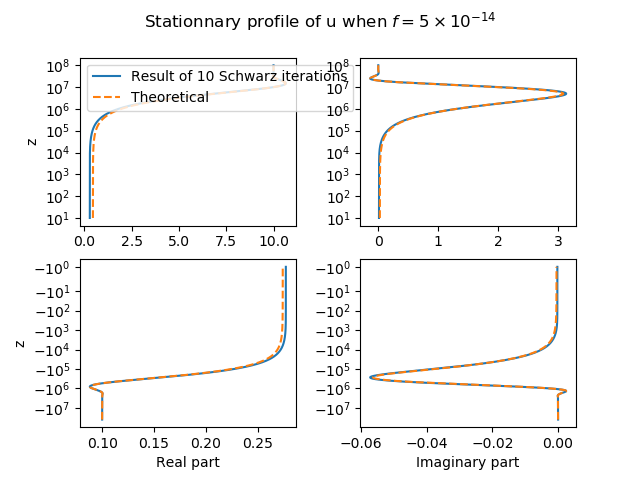
\includegraphics[scale=0.55]{profile_stationnaire_bug.png}
%     \caption{The validation works even if $y$ is not real: I don't understand why.
%     Wen we compute the modulus $x^2 + y^2$, we find a complex number, which makes no sense. This may explain the slight difference.}
%     \label{fig:profile_bug}
% \end{figure}
\subsection{Existence of solutions of the
non-linear semi-discrete in space problem}
\label{sec:OASchwarz_wellPosedness}
\cite{lions_mathematical_1995} proved the existence
of global in time weak solutions in
two dimensions with non-linearities inside the
computational domains but with a linear
interface condition.
We focus here on showing the existence of strong
unsteady solutions of the semi-discrete in space
problem with a non-linear interface condition.
In \citep{chacon-rebollo_existence_2014},
the existence of unsteady solutions of
non-linear turbulent models for oceanic surface mixing layers is
proven with the help of the inverse function theorem.
We will follow their method which is in three steps:
\begin{enumerate}
	\item showing the existence of a steady-state;
	\item showing the well-posedness of the linearized problem
	around the equilibrium;
	\item using of the inverse function theorem;
\end{enumerate}
The method can be generalized to other types of
non-linearities. In particular, we can show the existence and
uniqueness of problem \eqref{eq:SWRbulk}
(ignoring the Schwarz iteration indices) close to the
equilibrium state.
\begin{enumerate}
	\item The existence of a steady state is discussed above
		in this section.
	\item The well-posedness of the linearized
		problem is discussed in Appendix
	\ref{sec:OASchwarz_appendix_discreteVariationParameters}.
	\item The use of the inverse function theorem can be
		done in four steps:
	\begin{enumerate}
		\item concatenate the state vectors
			in a single vector $\mathbf{U}=
			\{u_a, u_o, \left.\phi_a\right|_{z=0}\}
			\in \mathbf{\cal U}$
		where $\mathbf{\cal U} = L^2([0,T])^{M_a+M_o+1}$.
		\item
	Define a mapping
	$\mathbf{\Phi}: \mathbf{\cal U}\rightarrow \mathbf{Y}$
	such that
\begin{equation}
	\label{eq:OASchwarz_wellPosedness_Phi}
\begin{aligned}
	\mathbf{\Phi}(\mathbf{U}) =
	\{&(\partial_t + if) u_a - \nu_a\partial_z \phi_a - g_a, \\
	&(\partial_t + if) u_o - \nu_o\partial_z \phi_o - g_o, \\
	&u_a(H_a, t) - u^\infty_a, ~~ u_o(H_o, t) - u^\infty_o, \\
	&\nu_{\rm a}\left.\phi_{\rm a}\right|_{z=0} - \alpha
	\left( U_{\rm a}\left(\frac{h_{\rm a}}{2},
	t\right) - U_{\rm o}\left(-\frac{h_{\rm o}}{2},
	t\right)\right) \\
	&\left.u_a\right|_{t=0} - U^e_{a}, ~~
	\left.u_o\right|_{t=0} - U^e_{o}\}
\end{aligned}
\end{equation}
where $\left.\phi_j\right|_{z\neq 0} = \partial_z u_j$
and $\partial_z$ is to be undertood as the finite difference
operator which is applied only where it makes sense:
for instance the first line of \eqref{eq:OASchwarz_wellPosedness_Phi}
is not applied for $z=H_a$.
Let us draw some important remarks about $\mathbf{\Phi}$:
\begin{itemize}
 \item The equation $\phi_o = \epsilon \frac{\nu_a}{\nu_o}\phi_a$
	 at interface is implicit;
 \item $\mathbf{\Phi}(\mathbf{U}^e)=0$
 	where $\mathbf{U}^e$
 	is the steady-state;
 \item the codomain $\mathbf{Y}$ is
 	\begin{equation}
		\mathbf{Y}=L^2([0,T])^{M_a-1}
			\times L^2([0,T])^{M_o-1}
 			\times L^2([0,T])^{3}
			\times \mathbb{R}^{M_a+M_o}
 	\end{equation}
\item 
finding $\mathbf{\Phi}^{-1}(y)$ is equivalent
to solving the nonlinear semi-discrete problem
\eqref{eq:SWRbulk} if the component of $y$ corresponding
to the interface condition is zero.
The idea of the proof is that if $\mathbf{\Phi}$ is invertible
around $\mathbf{U}^e$ then the nonlinear semi-discrete problem
\eqref{eq:SWRbulk} is invertible.
Moreover, the inverse function theorem also tells us that
$\mathbf{\Phi}^{-1}$ is continuous:
this means that around
the equilibrium state, the problem \eqref{eq:SWRbulk} is well-posed:
it has a unique solution that depends continuously
on the initial data.
\end{itemize}
	\item Show that $\mathbf{\Phi}$ is $C^1$ in a
		neighborhood of $\mathbf{U}^e$.
		First, note that the mapping
		$x \mapsto |x|x$ is analytic in a
		ball that does not contain zero.
		Then, $\mathbf{\Phi}$ is linear
		except for the part corresponding
		to the non-linear transmission condition.
		It is then straightforward to show that
		$\mathbf{\Phi}$ is $C^1$ and that
		its differential
		$D\mathbf{\Phi}(\mathbf{U}^e)$ is given
		by the linearized problem (a rigourous
		proof that can be directly adapted here
		is given in \cite{chacon-rebollo_existence_2014}).
		\item Show that $D\mathbf{\Phi}(\mathbf{U}^e)$
		is an isomorphism:
		$D\mathbf{\Phi}(\mathbf{U}^e)$ can
		be inverted by solving the linearized problem
		with additional input data.
		It is shown
		that it is well-posed in appendix
		\ref{sec:OASchwarz_appendix_discreteVariationParameters}.
	\end{enumerate}
\end{enumerate}

%====================================================
\section{Convergence analysis} \label{sec:conv-lin}
%====================================================
In this section we conduct a convergence analysis of the SWR algorithm 
\eqref{eq:SWRbulk} first with $\alpha$ a constant and then in a more 
complicated case where the problem is linearized around its 
equilibrium solutions. In the following we systematically make the assumption 
that the space domain is of infinite size (i.e. $H_j\to\infty$).
%====================================================
\subsection{Linear friction case ($\alpha = {\rm const}$)}
%\\[3mm]
%\textbf{Linear friction case ($\alpha = {\rm const}$)}\hspace*{5mm} %\label{sec:lin-analysis}
%%====================================================
%
%\subsubsection{Derivation of the convergence rate}
%
We assume in this paragraph that $\alpha=\alpha_{c}$ with $\alpha_{c}$ 
a constant independent of $U_j$ and we study the system satisfied by the errors
(i.e. $g_j, U_0, U^\infty =0$). 
%A Fourier transform makes a frequency variable $i\omega$ appear to characterise the 
%derivation in time.
The Fourier transform in time of the finite difference scheme
\eqref{eq:spaceTimeScheme}, together with an analysis
of the convergence as it was done in
Chapters \ref{ch:discreteSchwarzAnalysis} and
\ref{ch:approximatedDiscreteSchwarz}
%yields  
%$\widehat{U}_{{\rm a}, m+\frac{1}{2}}(\omega) =
%A_k(\omega) (\lambda_{\rm a}(\omega)+1)^m$
%%$\widehat{U}_{\rm a}(h_{\rm a}/2) = \nu_{\rm a} \frac{\widehat{\phi}_{\rm a}(h_{\rm a}) - \widehat{\phi}_{\rm a}(0)}{i(\omega+f) h_{\rm a}}$
%with $\omega \in \mathbb{R}$ the frequency variable. 
%After simple algebra, the transmission condition 
%\eqref{eq:bulkInterfaceCondition} in Fourier space expressed 
%in terms of the $\widehat{\phi}_j$ is 
%%////////////////////////////////////////////////////
%\begin{equation} \label{eq:discreteBulkFourier}
%\begin{aligned}
% \left( \frac{\chi_a\nu_a}{h_a}+\theta \alpha_c \right) \widehat{\phi}^k_{\rm a}(0) - \theta \alpha_c
%\widehat{\phi}^k_{\rm a}(h_a) = &(1-\theta) \alpha_c 
%(\widehat{\phi}^{k-1}_{\rm a}(h_{\rm a}) - \widehat{\phi}^{k-1}_{\rm a}(0)) \\
%&- \alpha_c \frac{h_a \nu_o}{h_o \nu_a} (\widehat{\phi}^{k-1}_{\rm o}(0) - \widehat{\phi}^{k-1}_{\rm o}(-h_{\rm o}))
%\end{aligned}
%\end{equation}
%with $\chi_j=\frac{i (\omega+f) h_j^2}{\nu_j}$.
%A discrete analysis of the finite difference scheme \eqref{eq:spaceTimeScheme} in the
(see Section \ref{appendix:OASchwarz_LinearizedAnalysis}
for a detailed derivation in the linearized case) leads to 
$\widehat{u}_{{\rm o}, -m - \frac{1}{2}}^k = A_k (\lambda_{\rm o}+1)^m$
and
$\widehat{u}_{{\rm a}, m + \frac{1}{2}}^k = B_k (\lambda_{\rm a}+1)^m$ 
with $\lambda_j = \frac{1}{2}\left(\chi_j - \sqrt{\chi_j} \sqrt{\chi_j + 4}\right)$,
$\chi_j=\frac{i (\omega+f) h_j^2}{\nu_j}$,
and $m$ the space index. The convergence factor of SWR is then
the rate at which $A_k$ or $B_k$ tends to 0.
The Fourier transform in time of the interface
transmission conditions gives
the evolution of $B_k$ which eventually leads to 
the following convergence factor: 
\begin{equation} \label{eq:cvBk}
\xi = \left|\frac{B_k}{B_{k-1}}\right| = 
\left|
	\frac{1 - \theta - \epsilon \frac{\lambda_{\rm a} - \chi_{\rm a}}
		{\lambda_{\rm o}} \frac{\nu_{\rm a} h_{\rm o}}
			{\nu_{\rm o} h_{\rm a}}}
	{\frac{\nu_a}{\alpha_c h_a}
	\left(\lambda_a - \chi_a \right)
	- \theta}
\right|
\end{equation}
%!!!!!!!!!!!!!!!!!!!!!!!!!!!!!!!!!!!!!!!!!!!!!!!!!!!!!!
%\begin{equation} \label{eq:cvBk}
%\xi = \left|\frac{B_k}{B_{k-1}}\right| = 
%\left|\frac{
%\left(1-\theta\right)
%+ \epsilon\frac{\lambda_{\rm o}}{\lambda_{\rm a}}
%}{
%\frac{i (\omega+f) \rho_{\rm a}h_{\rm a}}{\alpha\lambda_{\rm a}} %- \theta}\right|
%\end{equation}
%!!!!!!!!!!!!!!!!!!!!!!!!!!!!!!!!!!!!!!!!!!!!!!!!!!!!!!
% plot | (1-t) (((1+x^2)^(1/4) e^(-i atan(x)/2) - 1)) + ((1+(0.1 x)^2)^(1/4) e^(-i atan(0.1 x)/2)-1)|/| t (((1+x^2)^(1/4) e^(-i atan(x)/2) - 1)) - 1|, 0<t<1, 0<x<100
where $\epsilon = \frac{\rho_{\rm a}}{\rho_{\rm o}} \approx 10^{-3}$
in the ocean-atmosphere  context.
Note that the convergence factor \eqref{eq:cvBk} differs significantly from the semi-discrete convergence factor 
$\xi_{\rm DNWR} = \left|1 - \theta_{\rm DNWR} \left(
1 - \epsilon h_{\rm a} \lambda_{\rm o} / (\lambda_{\rm a}h_{\rm o})\right) \right|$ of 
the DNWR algorithm. 
Moreover, $\lambda_j$ is equivalent to $-\sqrt{\chi_j}$ when
$(\omega+f) \rightarrow 0$ and
as $(\omega+f) \rightarrow \infty$ we have
$\lambda_j\rightarrow -1$ and
$|\lambda_a - \chi_a| \rightarrow \infty$. The asymptotes
of $\xi$ for$(\omega+f) \rightarrow 0$ and
$(\omega+f) \rightarrow \infty$ are finally
\[
 \underset{(\omega+f) \rightarrow 0}{\mathrm{lim}} \xi = \frac{1}{\theta} \left| 1-\theta-\epsilon \sqrt{\frac{\nu_{\rm a}}{\nu_{\rm o}}}  \right| = \xi_0, \qquad
 \underset{(\omega+f) \rightarrow \infty}{\mathrm{lim}} \xi =
 \epsilon \frac{\nu_a h_o}{\nu_o h_a}.
\]
%\subsubsection{Asymptotic values for linear case}
As $\omega + f \to 0$ the asymptotic value 
$\xi_0$ depends on $\theta$: it is $+\infty$ for $\theta=0$ (i.e. a fast divergence), and $\xi_0 = \epsilon\sqrt{\frac{\nu_{\rm a}}{\nu_{\rm o}}}$ for $\theta=1$.
When $\omega\to \infty$, the convergence factor tends to a small value
that does not depend on $\theta$
(i.e. the convergence is rather fast for high frequencies).
% \\[3mm]
% \myTD{TODO relire la suite pour vérifier que c'est compatible
% avec cette expression là}
% \textbf{$\xi_0$ is an upper bound of the convergence factor in the linear friction case.}\hspace*{5mm} %\label{sec:lin-analysis}
% \begin{itemize}
%     \item From the definition of $\lambda_j$, we get that $\mathfrak{R}(\frac{\nu_{\rm a}\chi_{\rm a}}{\alpha_c h_{\rm a} \lambda_{\rm a}}) \leq 0$: the modulus of the denominator in \eqref{eq:cvBk} is hence greater than $\theta$.
%     \item For whatever frequency $\omega$, it seems that $\left|\frac{\lambda_j \sqrt{\nu_j}}{h_j}\right|$ increases with $\frac{\sqrt{\nu_j}}{h_j}$.
%     Indeed, we have that
% 	\begin{equation}
% 	\left|\frac{\lambda_j \sqrt{\nu_j}}{h_j}\right|
% 		= |\omega + f| |x - \sqrt{x}\sqrt{x+i}|,
% 		~~~~~ x = \frac{4}{i \chi_j} \in \mathbb{R}
% 	\end{equation}
% 	where the square root function is extended to the
% 		negative axis with $\sqrt{-|x|} := i\sqrt{|x|}$.
% 	The function $x \mapsto |x - \sqrt{x}\sqrt{x+i}|$
% 		seems to increase with $|x|$
%     (see Figure \ref{fig:figboundbulk}). It follows that if
% 	$\sqrt{\frac{\nu_{\rm o}}{\nu_{\rm a}}} \leq
% 		\frac{h_{\rm o}}{h_{\rm a}}$
% \begin{equation}
%     |1-\theta+\epsilon \frac{h_a \lambda_o}{h_o \lambda_a}| \leq | 1 - \theta| + \epsilon |\frac{h_a \lambda_o}{h_o \lambda_a}| \leq 
%     |1 - \theta| + \epsilon \frac{\sqrt{\nu_{\rm a}}}{\sqrt{\nu_{\rm o}}}.
% \end{equation}
% \end{itemize}
% \begin{figure}
%     \centering
%     \includegraphics[scale=0.6]{boundbulk.pdf}
%     \caption{Plot of the real function
% 	$x \mapsto |x - \sqrt{x}\sqrt{x+i}|$:
% 	 it decreases for $x<0$ and increases for $x>0$. A routine
% 	 computation tells that its derivative is asymptotically
% 	 positive for $x\rightarrow+\infty$.
% 	 % to do the routine computation:
% 	 % use that
% 	 % |x - \sqrt{x}\sqrt{x+i}|^2 = (x - \sqrt{x}\sqrt{x+i}) \times
% 	 %					(x - \sqrt{x}\sqrt{x-i})
% 	 % develop, and differentiate.
% 	 }
%     \label{fig:figboundbulk}
% \end{figure}
% For $\theta \leq 1$ and if 
% $\sqrt{\frac{\nu_{\rm o}}{\nu_{\rm a}}} \leq \frac{h_{\rm o}}{h_{\rm a}}$
% (the latter condition being easily satisfied), 
% the value $\xi_0$ is an upper bound 
% of the convergence factor.
Since we have $\epsilon \approx 10^{-3}$, 
the convergence is fast for $\theta = 1$ whereas $\epsilon$
does not play any role for $\theta = 0$
for which the Schwarz method does not converge.
%
%For $\theta=1$ and for typical values $\rho_a = 1\;{\rm kg}\;{\rm m}^{-3}$ the ratio $\frac{\rho_{\rm a}}{\rho_{\rm o}} \approx 10^{-3}$ accelerates the convergence, whereas its role when $\theta=0$ is limited.
%The dependency with regard to $\frac{h_{\rm a}}{h_{\rm o}}$ and to $\frac{\nu_{\rm a}}{\nu_{\rm o}}$ are
%harder to study because they depend on
%the variables involved in the ratios.
The optimal parameter $\theta_{\rm opt}$ for low frequencies is $1 - \epsilon\sqrt{\frac{\nu_{\rm a}}{\nu_{\rm o}}}$ which is very close to $1$.
\begin{remark}
	The asymptotes are different in \citep{clement_discrete_2021}.
	The mistake made in the authors' previous work
	is to consider the convergence factor of
	$(\phi_k)_{k\in \mathbb{N}}$
	whereas $\phi_k\to 0$ as $\omega+f\rightarrow 0$.
\end{remark}
%for parameter values 
%typical of the ocean-atmosphere coupling problem.
% The asymptotic value when $f\neq 0$ is
%\begin{equation}
%    \xi \to \left|\frac{1 - \theta +
%    \frac{\rho_{\rm a} \nu_{\rm a}h_{\rm o} }{\rho_{\rm o} \nu_{\rm o}h_{\rm a}}
%    \frac{1-\sqrt{1-i\frac{4\nu_{\rm o}}{f h_{\rm o}^2}}}{1-\sqrt{1-i\frac{4\nu_{\rm a}}{f h_{\rm a}^2}}}
%    }{\frac{\rho_{\rm a}\nu_{\rm a} h_{\rm a}}{\alpha \left( 1-\sqrt{1-i\frac{4\nu_{\rm a}}{f h_{\rm a}^2}}\right)} - \theta}\right|
%\end{equation}
%And setting the numerator to zero gives an approximation of $\theta_{\rm opt}$.
%However, the asymptotic value is no longer a bound of the convergence rate (
%The convergence rate when $\omega \to -f$ is the upper bound).
%==============================================================
%\\[2mm]
%\textbf{Linearized quadratic friction case}\hspace*{5mm}
\subsection{Linearized quadratic friction case}
%\label{subsec:linearized}
The analysis of the nonlinear quadratic friction case (i.e. with $\alpha = C_D\left|\right.U_{\rm a}\left(h_{\rm a} / 2, t\right) - U_{\rm o}\left(- h_{\rm o}/2, t\right)\left.\right|$)
cannot be directly pursued through a Fourier transform.
%Indeed $\alpha^k$ would still be expressed as a function of time while the variables $\widehat{\phi}$
%would depend on the frequency.
We thus consider the linearization of the problem 
around a steady state $U^e_j, \phi^e_j$ satisfying \eqref{eq:cplProblem}:
assuming that $U^k_j (\pm h_j/2, t)$ is in a neighborhood of $U^e(\pm h_j/2)$, the modulus in $\alpha$
is non-zero and
we can differentiate $\alpha$.
Differences with the steady state are noted $\delta \phi_j^k = \phi^k_j(0,t) - \phi_j^e(0)$ and $\delta U_j^k = U_j^k(\pm h_j/2, t) - U^e_j(\pm h_j/2)$.
\paragraph{Linearization of the transmission condition}
We will now linearize the transmission operator.
First, $\alpha^{k-1} \left(\delta U_a^{k-1+\theta}
- \delta U_o^{k-1}\right)$
is split into two parts in the non-linear transmission condition:
\begin{equation}
	\nu_a \phi_a^k =
	\underbrace{
	\alpha^{k-1} \left(\left(U^e_{\rm a} - U^e_{\rm o}\right) +
	\left(\delta U_a^{\emphase{k-1}}
	- \delta U_o^{k-1}\right)\right)}_{C_D|\cdot|(\cdot)}
	+ \emphase{\theta} \alpha^{k-1}
	\left(\delta U_a^{\emphase{k}} - \delta U_a^{\emphase{k-1}}
	\right)
\end{equation}
The transmission condition is linearized as
\begin{equation}
	\nu_a \delta \phi_a^k = \left\langle
	D_{\left(U_{\rm a}^e - U_{\rm o}^e\right)}
	C_D |\cdot|(\cdot),
	\left(\delta U_{\rm a}^{k-1} -
	\delta U_{\rm o}^{k-1}
	\right)
	\right\rangle
	+ \theta \alpha^{k-1}
	\left(\delta U_a^{k} - \delta U_a^{k-1}
	\right)
\end{equation}
where $D$ denotes the total derivative.
Let us first compute the total derivative of $x\mapsto |x|x$.
The total derivative of $|\cdot|^2$ is
\begin{equation}
\langle D_x |\cdot|^2, \mu \rangle
= \overline{x} \mu + x \overline{\mu}
\end{equation}
where $\overline{x}$ is the complex conjugate of $x$.
We then use the chain rule to differentiate $|x| = \sqrt{|x|^2}$ and
obtain
\begin{equation}
\langle D_x |\cdot|, \mu \rangle =
\frac{1}{2} \frac{\overline{x}}{|x|} \mu
+ \frac{1}{2} \frac{x}{|x|} \overline{\mu}
\end{equation}
Finally, the total derivative of the map $x\mapsto |x|x$ reads
\begin{equation}
	\langle D_x |\cdot|(\cdot), \mu \rangle =
	\frac{1}{2} \underbrace{\frac{\overline{x}x}{|x|}}_{=|x|} \mu
	+ \frac{1}{2}
	\underbrace{\frac{x^2}{|x|}}_{=|x|\frac{x}{\overline{x}}}
	\overline{\mu}
	+ |x|\mu
	= |x| \left(\frac{3}{2}\mu + \frac{1}{2}\frac{x}{\overline{x}}
	\overline{\mu}\right)
\end{equation}
Finally, the linearized transmission operator reads
%==========================================
\begin{equation}
\label{eq:linearised}
\begin{aligned}
\nu_{\rm a}\delta\phi_{\rm a}^k = \alpha^e 
\left( \left(\frac{3}{2} - \theta \right)\delta U_{\rm a}^{k-1} \right.
&+ \theta\, \delta U_{\rm a}^{k}
- \frac{3}{2} \delta U_{\rm o}^{k-1}
\\
&\left.+ \frac{1}{2}\frac{U_{\rm a}^{{\color{black} e}} - U_{\rm o}^{{\color{black} e}}}
	{\overline{U_{\rm a}^{{\color{black} e}} - U_{\rm o}^{{\color{black} e}}}}\,
\overline{
\delta U_{\rm a}^{k-1} - \delta U_{\rm o}^{k-1}}
\right)
\end{aligned}
\end{equation}
%==========================================
with $\alpha^e=C_D\left|U_{\rm a}^e(h_{\rm a}/2) - U_{\rm o}^e(-h_{\rm o}/2)\right|$.
\paragraph{Convergence study with the linearized transmission condition}
Following the derivation in the previous paragraph (detailed in
Section \ref{appendix:OASchwarz_LinearizedAnalysis} with
space domains of finite size),
we find that the evolution of $B_k$ is:
\begin{equation}
	\label{eq:OASchwarz_ConvergenceAnalysis_linearizedCV}
	B_{k+1}(\omega) = a_1(\omega) B_{k}(\omega) + a_2(\omega)
		\overline{B_{k}(-{\omega})}
\end{equation}
where $a_1, a_2 \in \mathbb{C}$ are defined in
Section \ref{appendix:OASchwarz_LinearizedAnalysis}.
% with $\epsilon = \frac{\rho_{\rm a} h_{\rm a}}{\rho_{\rm o} h_{\rm o}}$ 
% and $\mathcal{O} = 
% \frac{U_{\rm a}^e - U_{\rm o}^e}{\overline{U_{\rm a}^e - U_{\rm o}^e}} \frac{\omega+f}{\omega - f}$.
Note that the variable $\overline{i \omega}=-\omega$ appears when using the Fourier
transform on $\overline{\delta U_a^{k-1} - \delta U_o^{k-1}}$.
As a consequence,
the convergence factor $\xi^q$ in the linearized 
quadratic friction case differs from one iteration to another:
it is a function of
$\frac{\overline{B_{k-1}(-\omega)}}{B_{k-1}(\omega)}$.
% \paragraph{Asymptotic ($\omega+f \rightarrow 0$) convergence for
% 	one iteration}
% However, for $(\omega+f) \rightarrow 0$ the term 
% $\displaystyle \frac{1}{2}\frac{U_{\rm a}^e - U_{\rm o}^e}{\overline{U_{\rm a}^e - U_{\rm o}^e}}\,
% \overline{
% \delta U_{\rm a}^{k-1} - \delta U_{\rm o}^{k-1}}$
% vanishes, therefore the asymptotic convergence 
% rate $\xi_0^q$ is independent of the iterate:
% \[
%  \underset{(\omega+f) \rightarrow 0}{\mathrm{lim}} \xi^q = \frac{1}{\theta} \left| \frac{3}{2}-\theta+\frac{3}{2}\epsilon\sqrt{\frac{\nu_{\rm a}}{\nu_{\rm o}}} \right| = \xi_0^q, \qquad
%  \underset{(\omega+f) \rightarrow \infty}{\mathrm{lim}} \xi^q = 0.
% \]
% The convergence is fast for high frequencies,
% as in the linear friction case. However
% the optimal parameter for $(\omega+f) \rightarrow 0$ is
% here $\theta_{\rm opt}^q = \frac{3}{2} +
% \frac{3}{2}\epsilon\sqrt{\frac{\nu_{\rm a}}{\nu_{\rm o}}}$.
% It is different from the optimal parameter $\theta_{\rm opt}$
% obtained with linear friction: for typical values of the
% ocean-atmosphere coupling problem, $\theta_{\rm opt}^q$
% is close to $\frac{3}{2}$.
% The asymptotic value $\xi_0^q$ is not an upper bound of the
% convergence factor but it is a good choice for $\theta_{\rm opt}^q$,
% as shown in the numerical experiments in Section \ref{sec:num-exp}.
% \par
% The asymptotic behavior for $\omega+f \rightarrow 0$ with
% multiple iterations differs from the asymptotic convergence
% rate $\xi_0^q$ above:
% indeed, $B_{k+1}(\omega)$ depends on
% $\overline{B_k(- \omega)}$ which itself depends on
% $\overline{\mathcal{O}(-\omega)} B_{k-1}(i\omega)$
% which could explode because
% $|\overline{\mathcal{O}(-\omega+ f \rightarrow 0)}|
% \rightarrow \infty$.
% \paragraph{Non-asymptotic convergence}
% If multiple iterations are performed,
We need to look at both
$B_{k+1}(\omega), \overline{B_{k+1}(-{\omega})}$
at the same time:
\begin{figure}
    \centering
    \includegraphics[scale=0.65]{plotEigenvaluesValidated.pdf}
	\caption{Singular values $\widetilde{\xi}_1(\omega)$,
	$\widetilde{\xi}_2(\omega)$ of the matrix $\begin{pmatrix}
	a_1(\omega) & a_2(\omega) \vspace{0.15cm}\\
	\overline{a_2(-\omega)} & \overline{a_1(-\omega)} \\
	\end{pmatrix}$.
	The observed "convergence factor" at the first
	iteration ${\xi}_{\rm obs} = \sqrt{\frac{|B_2(\omega)|^2 +
	|B_2(-\omega)|^2}{|B_{1}(\omega)|^2
	+ |B_{1}(-\omega)|^2}}$
	is in purple. ${\xi}_{\rm obs}$ is such that
	$\widetilde{\xi}_2 \leq {\xi}_{\rm obs}
	\leq\widetilde{\xi}_1$ (see Figure
	\ref{fig:OASchwarz_rateBetweenEigenvalues}).
	}
    \label{fig:OASchwarz_singularValues}
\end{figure}
\begin{equation}
	\begin{aligned}
		B_{k+1}(\omega) &= a_1(\omega) B_{k}(\omega) + a_2
		\overline{B_{k}(-{\omega})}\\
		\overline{B_{k+1}(-{\omega})} &=
		\overline{a_1(-{\omega})
			B_{k}(-{\omega})
		+ {a_2(-{\omega})} \overline{B_{k}(\omega)}}
	\end{aligned}
\end{equation}
\begin{figure}[htpb]
	\centering
	\scalebox{0.8}{
		\import{}{rate_between_eigenvalues.pdf_tex}}
	\caption[The convergence factor $\xi(k)$ varies and is bounded]{
	The vector
	$\mathbf{B}^k= \begin{pmatrix} B_k(\omega) \vspace{0.15cm}\\
	\overline{B_k(-\omega)} \end{pmatrix}$
	can be decomposed into a basis\footnotemark of eigenvector
	$\mathbf{B}_i^k$ which converge linearly with
	convergence factors $\widetilde{\xi}_i$.
	4 iterations are shematically represented in blue, pink,
	orange and purple. The "convergence factor"
	$\xi_{\rm obs}(k)=\frac{||\mathbf{B}^{k+1}||}{||\mathbf{B}^{k}||}$
	is such that
	$\widetilde{\xi}_2 \leq \xi_{\rm obs} \leq \widetilde{\xi}_1$ and
	varies from one iteration to another. $\xi(k)$
	gets closer to $\widetilde{\xi}_1$ when $k$ increases as
	$\mathbf{B}^k$ gets closer to $\mathbf{B}^k_1$.
	}
	\label{fig:OASchwarz_rateBetweenEigenvalues}
\end{figure}
\footnotetext{The matrix is indeed diagonalizable if
$\widetilde{\xi}_1 \neq\widetilde{\xi}_2$; otherwise we
have a simple convergence factor
$\xi = \widetilde{\xi}_1 = \widetilde{\xi}_2$.
}
We examine the evolution of those two
simulaneously evolving quantities:
\begin{equation}
	\label{eq:OASchwarz_transitionMatrixDD26}
\begin{pmatrix}
	B(\omega) \vspace{0.15cm}\\
	\overline{B(-{\omega})}
\end{pmatrix}_{k+1}
 =
\begin{pmatrix}
	a_1(\omega) & a_2(\omega) \vspace{0.15cm}\\
	\overline{a_2(-{\omega})} & \overline{a_1(-{\omega})} \\
\end{pmatrix}
\begin{pmatrix}
	B(\omega) \vspace{0.15cm}\\
	\overline{B(-{\omega})}
\end{pmatrix}_{k}
\end{equation}
The singular values (shown in Figure \ref{fig:OASchwarz_singularValues})
of the $2\times 2$ matrix
in \eqref{eq:OASchwarz_transitionMatrixDD26}
can be studied instead of the convergence factor.
One can see on Figure \ref{fig:OASchwarz_singularValues} that
the two singular values are different for small frequencies,
especially around the frequencies $f$ and $-f$.
\par
One can hence expect (see
Figure \ref{fig:OASchwarz_rateBetweenEigenvalues}) that for frequencies close to $f$ and $-f$
the "convergence factor"
$\sqrt{\frac{|B_k(\omega)|^2 +
|B_k(-\omega)|^2}{|B_{k-1}(\omega)|^2 + |B_{k-1}(-\omega)|^2}}$ will be
\begin{itemize}
	\item different from one iteration to another;
	\item between $\widetilde{\xi}_1$ and $\widetilde{\xi}_2$.
\end{itemize}
We optimize only the maximum over the frequencies of the biggest
singular value $\widetilde{\xi}_1$ (see Figure
\ref{fig:OASchwarz_nonasymptotic})
\begin{figure}
    \centering
    \includegraphics[scale=0.65]{asymptote_linearized.pdf}
	\caption{Singular values
	$\widetilde{\xi}_1, \widetilde{\xi}_2$ of $\begin{pmatrix}
	a_1(\omega) & a_2(\omega) \vspace{0.15cm}\\
	\overline{a_2(-\omega)} & \overline{a_1(-\omega)} \\
	\end{pmatrix}$ maximized over the set of discrete
	frequencies
	$\{-\frac{\pi}{\Delta t}, ..., \frac{\pi}{T}, 0,
	\frac{\pi}{T},..., \frac{\pi}{\Delta t}\}$.
	The vertical dashed line highlights the minimum
	of $\max \widetilde{\xi}_1$.
	The windows length $T$ is one day
	and $\Delta t=60\;{\rm s}$ .
	}
    \label{fig:OASchwarz_nonasymptotic}
\end{figure}
and find that the optimal value of $\theta$ is slightly smaller than
$1.5$ (instead of an optimal value slightly bigger than $1.5$
for the asymptotic convergence for one iteration)
\section{Numerical experiments}
\label{sec:num-exp}
% \begin{figure}
%     \centering
%     \includegraphics[scale=0.6]{localCvRate.pdf}
%     \caption{Local convergence rate $\frac{B_{k+1}}{B_{k}}$ where $k$ is on the vertical axis and the frequency $\omega$ on the horizontal axis. The convergence is faster as the color is brighter.}
%     \label{fig:localCvRate}
% \end{figure}
The aim of this section is to illustrate the influence of the parameter $\theta$, in the linear and quadratic friction cases. 
The steady state $U_j^e$ is used to compute $\alpha_c = \alpha^e = C_D|U_{\rm a}^e(\frac{h_{\rm a}}{2}) - U_{\rm o}^e (\frac{h_{\rm o}}{2})|$ in the linear case.
Parameters of the problem are taken as realistic: $C_D = 1.2\times 10^{-3}$, the space steps are $\frac{h_{\rm a}}{2} = 10\; {\rm m}$, $\frac{h_{\rm o}}{2} = 1 \;{\rm m}$,
the time step  is $60 \;{\rm s}$,
the size of the time window $T$ is 1 day ($1440\Delta t$) and the computational domains sizes are $H_o = H_a = 2000 \; {\rm m}$
(100 and 1000 nodes respectively in $\Omega_a$ and $\Omega_o$).
The Coriolis parameter is 
$f=10^{-4}\; {\rm s^{-1}}$ and the diffusivities are 
$\nu_{\rm a} = 1\; {\rm m^2}\;{\rm s}^{-1}, 
\nu_{\rm o} = 3\times 10^{-3} \;{\rm m^2}\;{\rm s}^{-1}$. 
 $U_j^\infty$
are  set to constant values of $10\;{\rm m}\;{\rm s}^{-1}$ in the 
atmosphere and $0.1\;{\rm m}\;{\rm s}^{-1}$ in the ocean, while the forcing terms 
$g_j=i f U^\infty_j$ and the initial condition $U_0(z)=U_j^e(z)$.
SWR is 
initialized at the interface with a white noise around the interface value
of the initial condition.
Figure \ref{fig:evolutionErrNonlinear} shows the evolution of the error for two choices of $\theta$. The theoretical
convergence according is
also displayed: $\sup_\omega \xi$ is an upper bound of the $L^2$ convergence factor \cite{thery_etude_2021}. In the case
$\alpha={\rm const}$ we use $\xi_0$ as an approximation of
$\sup_\omega \xi$.
The theoretical bounds $\max_\omega \widetilde{\xi}_1$ and $\xi_0$
fit rather accurately the convergence rate and one can see that
those values are indeed greater than the observed convergence rate.
Figure \ref{fig:evolutionErrNonlinear} confirms the results of Section \ref{sec:conv-lin}:
when considering $\alpha=\alpha_c$ constant, the fastest convergence is achieved when $\theta$ is close to 1, similarly to the DNWR algorithm.
However this does not translate into the nonlinear case, which converges faster with $\theta=1.5$.
Figure \ref{fig:robustesseEvolutionErrNonlinear}
shows that the convergence behavior with the linearized transmission condition is
similar to the nonlinear case.
As expected the convergence is faster for $\theta=1.5$
than for $\theta=1$.
We observed that those results are robust to changes in the values of the parameters in the range of interest.
%Numerical experiments with the linearized transmission condition converge at the same speed as with the nonlinear condition. 
Linearized transmission conditions are hence relevant to study
theoretically the
convergence properties of our nonlinear problem.
\begin{figure}
    \centering
    \includegraphics[scale=0.65]{evolution_err_nonlinear.pdf}
    \caption{Evolution of the  $L^2$ norm of the errors. Black lines represent the observed convergence; grey lines are the estimated convergence with slopes $\xi_0$ for linear cases and $\max_\omega \widetilde{\xi}_1$ for quadratic cases.}
    \label{fig:evolutionErrNonlinear}
\end{figure}
\begin{figure}
    \centering
    \includegraphics[scale=0.65]{robustesse_evolution_err_nonlinear.pdf}
    \caption{Evolution of the  $L^2$ norm of the errors with linearized (L) and nonlinear (NL) transmission conditions. The legend indicates the changes in the parameters for each case. }
    \label{fig:robustesseEvolutionErrNonlinear}
\end{figure}
%
\section{Conclusion}
In this paper, we studied a SWR %Schwarz Waveform Relaxation 
algorithm applied
to a simplified ocean-atmosphere problem. 
This problem considers nonlinear transmission conditions arising 
from wall laws representative of the ones used in Earth-System Models
and analogous to a quadratic friction law. We 
motivated the fact that the convergence analysis of such 
problems can only be done at a semi-discrete level in space due to the particular practical implementation of continuous interface conditions in actual climate models.  
The steady state of the coupled problem was derived analytically
and it was proven that the unsteady problem is well-posed
in a neighborhood of the steady state.
Then we analytically studied the convergence properties in a
case with linear friction and in a case with linearized 
quadratic friction. We formulated the problem with a 
relaxation parameter $\theta$ in the transmission conditions and 
systematically assessed its impact on the convergence speed. 
%
%
%We considered transmission conditions close to state-of-the-art handling of air-sea exchanges and compared the convergence speed of
%%SWR for linear and nonlinear versions of those conditions.
%We introduced a free parameter $\theta$ in the transmission condition that resembles %to a relaxation parameter, and showed that its choice is crucial for the speed of %convergence, for both linear and nonlinear conditions.
%
%Because the transmission conditions are entangled with the discretization, a semi-discrete in space analysis was conducted on SWR with the linear condition. 
%
For the two cases of interest, the convergence factors were derived
which allowed us to choose appropriate values
for the parameter $\theta$ to guarantee fast convergence of the algorithm.
%to indicate a parameter $\theta_{\rm opt}$ 
%The same asymptotic value was derived for the nonlinear transmission operator, linearized around a steady state.
%
The behavior of the algorithm for linear friction and linearized 
quadratic friction turns out to be different which leads to different
"optimal" values of $\theta$. 
%
%The parameter $\theta_{\rm opt}^q$ which is found is
%different from $\theta_{\rm opt}$, and 
%
Numerical experiments in the nonlinear case showed that the observed 
convergence behaves as predicted by the linearized quadratic friction
case.
